\chapter{Estado del arte}

Nuestra investigación parte de ideas pertenecientes a dos campos. El primero y la inspiración original para este
trabajo son las tecnicas de Style transfer y el otro son las herramientas de modelado. Puesto que,
nuestro objetivo final es generar una herramienta que permita convertir cualquier modelo tridimensional en algo que
se asemeje a una escultura gargallesca imitando un recurso caracteristico del escultor. Pero dandole al usuario la capacidad
de controlar en mayor grado las transformaciones y la edición que realiza sobre el modelo tridimensional.

\section{Style transfer}
El Style transfer es una tecnica que trata de generar una imagen nueva a partir del contenido de una imagen y el estilo de otra. Es decir, que
conserve el contenido de la imagen original mientras aplica el estilo visual de otra imagen.\cite{paperswithcodePapersWith} La forma mas extendida
en la que se ha utilizado esta tecnica es con imagenes. Habitualmente con cuadros de artistas como referencia de estilo. 
\begin{figure}
    \centering
    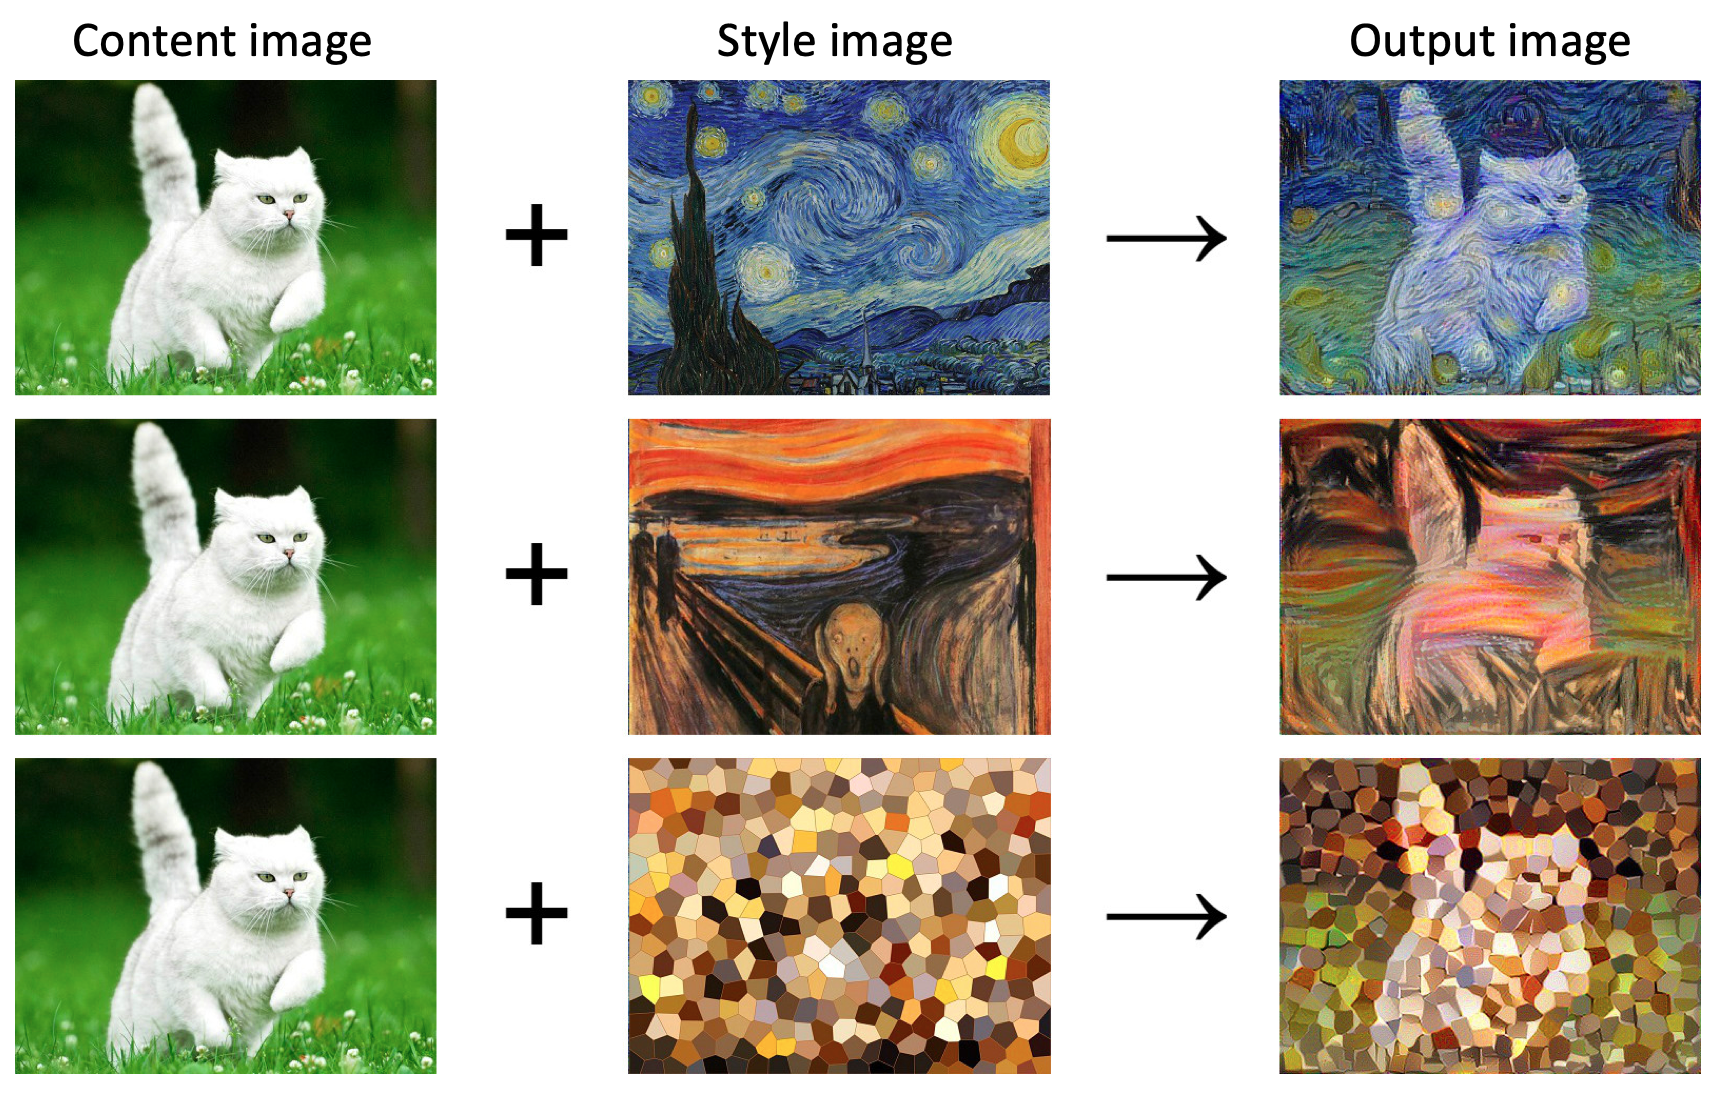
\includegraphics[width=\textwidth]{imagenes/style-transfer-example.jpg}
    \caption[Ejemplo de uso de Style Transfer]{Ejemplo de uso de Style transfer para pasar la imagen de un gato a diferentes estilos artisticos}
\end{figure}
Esto se ha consegudo hacer utilizando recursos del Aprendizaje automatico. Y existen varias formas de conseguirlo. La primera vez que se logro realizar una
transferencia de estilo fue utilizando redes neuronales con un acercamiento que trataba de utilizar una red neuronal cuyo objetivo era generar una imagen de salida
la cual tenia que minimizar una función compuesta por la suma de una función de perdida de estilo y una función de perdida de contenido. Estan funciones calculaban cuanto se habia alejado la imagen generada por la red neuronal
del estilo objetivo que estaba tratando de imitar, y cuanto se alejaba la imagen resultado del contenido de la imagen original respectivamente. De esta forma entrenamos una red neuronal tratando de cambiar ligeramente el valor de los
pixeles de la imagen de salida hasta que la función de evaluación converga o hasta que estemos satisfecho con el resultado. \cite{Gatys_2016_CVPR}. Sin embargo este acercamiento no es el unico que se utiliza para hacer style transfer.

Sin embargo este campo ha sufrido avances que estan empezando a permitir realizar estos cambios de estilo para modelos tridimensionales. Herramientas como 3DSNet \cite{segu20203dsnet} o PSnet \cite{Cao_2020_WACV} son avances novedosos que surgieron
durante el 2020 y tratan de acercar el enfoque de minimización de funciones de perdida de estilo y contenido que hemos descrito antes para las peculiaridades de las mallas tridimensionales. Trabajando sin embargo principalmente con nubes de puntos en
un espacio tridimensional. Esta representación de la geometria es de hecho bastante común y utilizada en casos reales como la conducción autonoma. Para la tarea de realizar una transferencia de estilo entre nubes de puntos tridimensionales PSnet utiliza
perceptrones multicapa para extraer la representación de la geometria y el color de la nube de puntos. Para ello Utiliza el acercamiento que ya utilizo PointNet\cite{PointNet}. El cual se basa en utilizar un Perceptron multicapa para expandir cada punto tridimensional a un espacio de caracteristicas
de mayor dimensionalidad para luego extraer información sobre esa red de puntos. Despues PSnet trata los valores intermedios del perceptron multicapa como una representación del contenido de la nube de puntos y se encarga de hacer que encaje con la codificación del estilo. De esta forma es capaz de generar una nueva
nube de puntos a partir de dos nubes de puntos de entrada diferentes. Una para representar el contenido de la nube de puntos de salida y otra para representar el estilo de la nube de puntos de salida. Por otro lado 3DSNet utiliza tecnicas mas avanzadas de aprendizaje profundo y se aleja un poco del enfoque que hemos explicado 
para ofrecer una alternativa a PSNet.

\begin{figure}
    \centering
    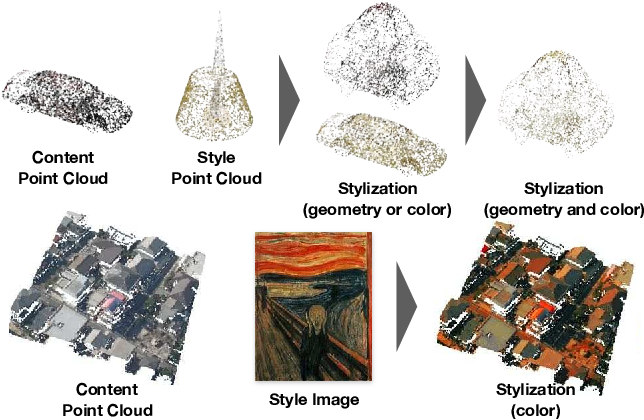
\includegraphics[width=\textwidth]{imagenes/FiguraPaper.png}
    \caption{Ejemplo del funcionamiento de PSNet \cite{Cao_2020_WACV}}
\end{figure}

\section{Herramientas de modelado tridimensional}

Este tipo de herramientas permiten a un usuario con los conocimientos necesarios para usarlas crear modelos tridimensionales. Normalmente estan diseñadas para un publico perteneciente al campo de las artes digitales. Para cumplir su cometido otorgan a sus usuarios herramientas que aunque de forma interna trabajan con las estructuras matematicas que definen un modelo tridimensional
para un ordenador se basan en conceptos e intuiciones mucho mas visuales. Permitiendo que los artistas puedan transferir los conocimientos y las tecnicas que ellos trabajan en el mundo físico al mundo digital. Podriamos catalogar nuestro trabajo como una de estas herramientas que ofrecen este tipo de programas. A dia de hoy existen muchas alternativas y Softwares de modelado tridimensional
usados en la industria. Programas como Autodesk Maya, Autodesk 3Ds Max, Houdini o Blender ofrecen soluciones de modelado y son ampliamente utilizados en la industria. Destacamos Blender pues de todos los que hemos mencionado es el unico que no es software propietario y por el contrario es un proyecto open source liberado bajo la licencia \cite{gplv3}. Esto permite que aunque existen varias organizaciones
como el Instituto de Blender o la Fundación Blender que se encargan del mantenimiento y desarrollo de la herramienta. El proyecto permite a su publico acceder y modificar libremente la base de codigo. Permitiendo a toda la comunidad desarrollar nuevas herramientas o arreglar bugs. \cite{blenderAboutBlenderorg}

